\chapter{Quantum Generative Adversarial Networks}\label{chapter:quantum_gans}
The field of Quantum Machine Learning (QML) is still in very early stages and there
has been an ongoing effort on translating the  classical Machine Learning (ML)
concepts into QML realm. Because of the limitations of current quantum computers
(NISQ) \cite{bharti2021noisy} and overall different paradigm of Quantum
Computing (QC), this process is difficult and there is no clear
answer to the question ``how this concept should be realized on QC device?''.
While in classical GANs generator and discriminator are realized as deep neural
networks, NISQ devices are not yet powerful enough to support such architecture.
Instead parametric quantum circuits \cite{Schuld_2020} are used.

In this chapter we take a closer look at two different designs of quantum GANs.
We briefly explain theory behind them and show the results of our evaluation.
The quantum GANs introduced in this chapter are the base of our hybrid
classical-quantum generative framework.

\section{Standard Quantum GANs (SQGANs)}
In the classical GANs, both the discriminator and generator are deep, general
purpose neural networks. The logical extension of this design in the quantum
realm is to model those are general purpose parametric quantum circuits. This
idea was formalized by Dallaire-Demers et al. \cite{Dallaire_Demers_2018} in
the architecture we call SQGANs (Figure \ref{fig:SQGANs_circuit}). The generator
starts in the state $\ket{0}^{\otimes n}$ in the \textbf{Our R/G} wire, where
$n$ is the dimension of the real quantum samples.
Additionally, the generator takes the label state $\ket{\lambda}$ in the
\textbf{Label R/G} wire and the random state $\ket{z}$ that provides the entropy in
the \textbf{Batch R/G} wire. The label state $\ket{\lambda}$ lets the
generator to learn the conditional distribution $p_g(x|\lambda)$ instead of $p_g(x)$,
this design was inspired by classical Conditional GANs
\cite{mirza2014conditional}. The discriminator takes the generated state
$\rho_\lambda^G$ or real state $\rho_\lambda^R$ and the corresponding label
$\ket{\lambda}$ in the \textbf{Label D} wire, it also uses the workspace
\textbf{Batch D} initialized in $\ket{0}$ state. The measurement on the single
qubit wire \textbf{Out D} corresponds to the probability of the state in 
\textbf{Out R/G} being real or generated.

There are not any particular restrains on how $G$ and $D$ circuits should look
like. However, to be able to learn and differentiate between arbitrary quantum
states the ansatz used should be universal (i.e. be able to generate every
quantum state given appropriate depth). The ansatz used in this
work is described in details in Appendix \ref{apx:sqgans_ansatz}.

\begin{figure}[htbp!]
  \begin{tikzcd}
    \rstick{Out D} &&&&&& \rstick{$\ket{0}$} &&& \qw & \qw & \gate[4, disable auto height]{D(\theta_D)} & \meter{} \\
    \rstick{Batch D} &&&&&& \rstick{$\ket{0}^{\otimes d}$} &&& \qw & \qw & & \qw \\
    \rstick{Label D} &&&&&& \rstick{$\ket{\lambda}$} &&& \qw & \qw & & \qw \\ 
    \rstick{Out R/G} &&&&&& \rstick{$\ket{0}^{\otimes n}$} &&& \gate[3, disable auto height]{
      \begin{array}{c}
      R \\ or \\ G(\theta_G)
      \end{array}
    } & \qw \rho_{\lambda}^{R/G} & & \qw \\ 
    \rstick{Label R/G} &&&&&& \rstick{$\ket{\lambda}$} &&& \qw & \qw & \qw & \qw \\ 
    \rstick{Batch R/G} &&&&&& \rstick{$\ket{z}$} &&& \qw & \qw & \qw & \qw 
  \end{tikzcd}
  \caption{SQGANs schema. The discriminator $D$ and the generator $G$ are
    parametric quantum circuits. The first 3 wires go
    directly to the discriminator. \textbf{Out D} outputs the probability of the
  input being generated. \textbf{Batch D} is an additional workspace of the
  discriminator and \textbf{Label D} contains the label state. \textbf{Out R/G}
  carries the generated or real state. \textbf{Label R/G} contains the label
  state and \textbf{Batch R/G} is the noise source for the generator, not used
  with the real samples.\label{fig:SQGANs_circuit} }
\end{figure}

\subsection{Training}
As in the SGANs we are interested in the minmax game setting. Specifically, in
the \textbf{Out D} wire, the measurement of $\ket{1}$ indicates that the sample
was real and $\ket{0}$ that the state was generated by $G$.
\footnote{Using $\ket{1}$ and $\ket{0}$ in this order is just a convention we
  assume. Any other orthogonal pair can be used.}
This should be the case for each label state $\ket{\lambda}$, which gives the
objective \ref{eq:SQGANs_objective}. 
\begin{equation}
  \begin{split}
  \label{eq:SQGANs_objective}
  & \max_{D}\min_{G} \mathcal{L}(G, D) = \\
  & \max_{D}\min_{G}  \frac{1}{\Lambda}\sum_{\lambda \in \Lambda}{P((D(\theta_D, \ket{\lambda}, R(\lambda)) = \ket{1}) \land (D(\theta_D, \ket{\lambda}, G(\theta_G, \ket{\lambda}, \ket{z}) = \ket{0})))}
  \end{split}
\end{equation} 
Where the discriminator objective is to maximize the probability of measuring $\ket{1}$
given real sample and measuring $\ket{0}$ given generated state. At the same
time for the generator the objective is to do the opposite.

The SQGANs cost function \ref{eq:SQGANs_objective} in contrast to the SGANs cost
function \ref{eq:SGANs_objective} is not defined with log-likelihood. In quantum
setup is more natural to work with linear functions and since the $\log$ is
convex, the optimum is the same for both.

The cost function $\mathcal{L}(G, D)$ expressed in terms of measurements and
assuming equal probability of sampling from $R$ and $G$ takes the form \ref{eq:SQGANs_objective}

\begin{equation}
  \label{eq:SQGAN_objective_trace}
  \mathcal{L}(G, D) = \frac{1}{2} + \frac{1}{4\Lambda}\sum_{\lambda \in
  \Lambda}{}tr((\rho_\lambda^{DR}(\theta_D) - \rho_\lambda^{DG}(\theta_D, \theta_G, z))Z)
\end{equation}
For detailed derivation on how to get from \ref{eq:SQGANs_objective} to
\ref{eq:SQGANs_objective} refer to Appendix \ref{apx:sqgans_cost_function}.

\subsubsection{Gradient Estimation}
To optimize the parameters $\theta_D$ and $\theta_G$ classical gradient descent
method was used. First, the value of the cost function $\mathcal{L}(G, D)$ was
estimated by sampling from the circuit \ref{fig:SQGANs_circuit}. This allows to
calculate the gradient w.r.t. $\theta_D$ and $\theta_G$ on classical computer
and update the parameters at the step $k$ in the following way
\begin{equation}
  \begin{split}
    \theta^{k+1}_D = \theta^{k}_D + \alpha^k_D\nabla_{\theta_D}\mathcal{L}(\theta^k_G, \theta^k_D) \\
    \theta^{k+1}_G = \theta^{k}_G - \alpha^k_G\nabla_{\theta_G}\mathcal{L}(\theta^k_G, \theta^k_D)
  \end{split}
\end{equation}
where $\alpha^k_D$ and $\alpha^k_G$ are learning rate metaparameters that can
depend on the step $k$.

It is also possible to estimate the gradient directly on quantum computer by
creating an explicit quantum circuit for each element of vectors $\theta_D / \theta_G$
and reading the grading by sampling for those circuits \cite{Dallaire_Demers_2018}.
\subsection{Evaluation Results}
\subsubsection{Experimental Setup}
In all of the experiments the real samples are generated by evaluating the
circuit from Figure \ref{fig:phase_circuit_small}. This circuit was constructed
by Smith et al. \cite{smith2020crossing} to study topological phase transitions.
All the gates in the circuit are parameterized by a single real valued parameter
$g \in [-1;1]$. The detailed gates layout is described in Appendix \ref{apx:topological_phase_transition_ansatz}.
\begin{figure}[htbp!]
  \begin{tikzcd}
    \lstick{$\ket{0}$} & \gate[2, disable auto height]{U_1(g)} & \qw & \qw & \qw &
    \qw & \qw & \qw \\
    \lstick{$\ket{0}$} & & \gate[2, disable auto height]{U(g)}  & \qw & \qw & \qw & \qw & \qw \\
    \lstick{$\ket{0}$} & \qw & \qw & \gate[2, disable auto height]{U(g)}  & \qw & \qw & \qw & \qw \\
    \lstick{$\ket{0}$} & \qw & \qw & \qw & \qw & \ldots  \\
    \vdots & & & & &\ldots & \gate[2, disable auto height]{U(g)} & \qw \\
    \lstick{$\ket{0}$} & \qw & \qw & \qw & \qw & \qw & \qw & \qw \\
  \end{tikzcd}
  \caption{The circuit used for generating real samples. All the gates are
    parametrized by a real valued parameter $g \in [-1; 1]$. For detailed
    description of the circuit see Appendix
    \ref{apx:topological_phase_transition_ansatz} \label{fig:phase_circuit_small}}
\end{figure}

The generator and discriminator are both build using the generic circuit
architecture from Appendix \ref{apx:sqgans_ansatz}. The number of layers differs
and is specified for each experiment separately.

In all the experiment we use Adam optimizer \cite{kingma2017adam} with
parameters $\beta_1 = 0.9$, $\beta_2=0.98$, $\hat{\epsilon} = 1e-9$. The
learning rate is calculated as
\begin{equation}
lr = \max{(\exp{(-\frac{(k+200) * \ln{100}}{4000}), 0.01)}}
\end{equation}
where $k$ is the optimization step number. The
learning rate decreases from $\sim 0.8$ to $0.01$ in the first $3800$ steps and then
remains at $0.01$ for the rest of the training. The exact values were derived
experimentally and show overall good convergence. The exact number of epochs and
iterations is specified for each experiment separately.
\subsubsection{Results For Pure State Real Input}
In this setup the generator is fed the same real input state at every iteration.
The real input state is generated using circuit from Figure
\ref{fig:phase_circuit_small} for random $g \in [-1; 1]$.


In Figure \ref{fig:sqgans_res_3} we present the
results of experiments for different widths of the real input circuit. For All
the experiments, the generator and discriminator were built using ansatz
from Appendix \ref{apx:sqgans_ansatz} for each layer. The \textbf{Label} and
\textbf{Batch} wires are not used for any circuit.

For each real input width the generator was able to approximate the real source,
increasing the fidelity as the training progressed. The training was
harder for the bigger real source circuits and it can be clearly seen that
the results for wider inputs are worse. Not only the final fidelity is lower, but
also it fluctuates much more. It is also much harder for the generator to fool
the discriminator for wider inputs.

It is not surprising that it is more difficult to train circuits with more
qubits. We also acknowledge that with different metaparameters or optimization
method the results could be better. However, our best results for more than 5 qubits
in the real source are not longer useful for the real source approximation.

\begin{figure}[htbp!]
  \captionsetup[subfigure]{labelformat=empty}
  \centering
  \subfloat{
    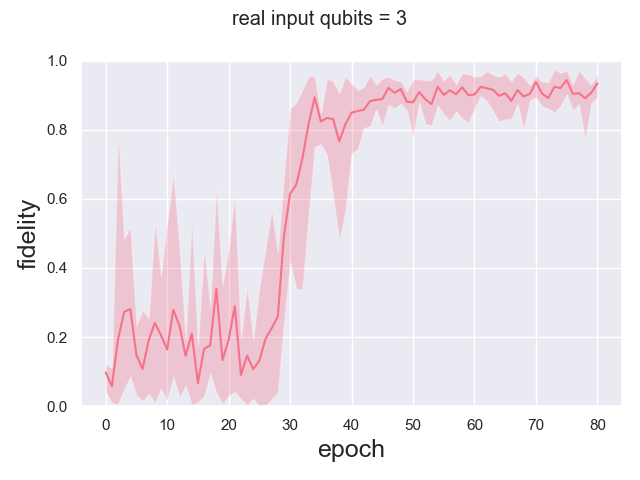
\includegraphics[width=0.3\linewidth]{figures/sqgans_size=3/fidelity.png}
  }
  \subfloat{
    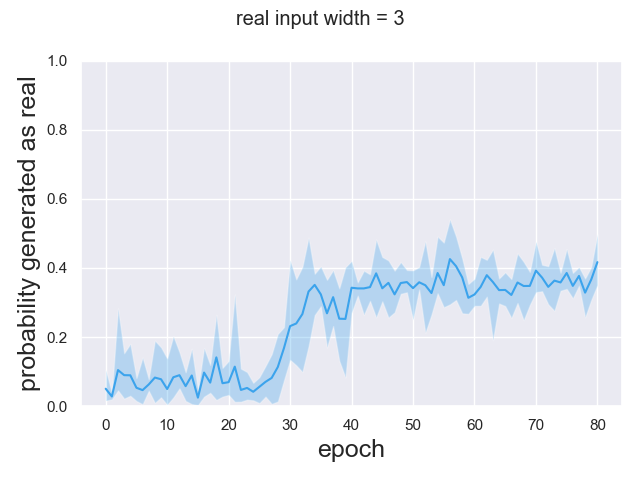
\includegraphics[width=0.3\linewidth]{figures/sqgans_size=3/probability_generated_as_real.png}
  }
  \subfloat{
    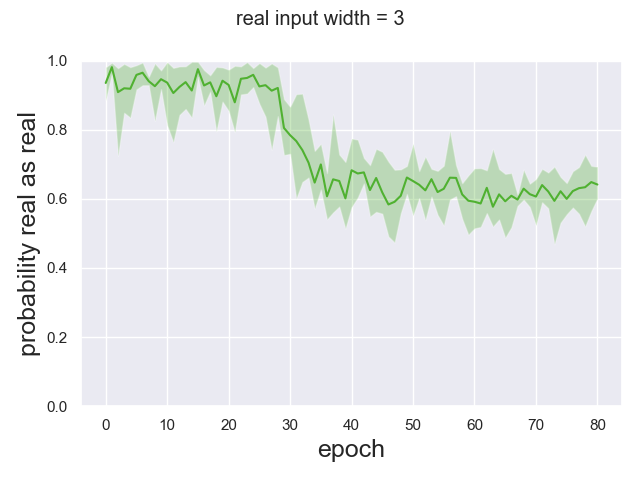
\includegraphics[width=0.3\linewidth]{figures/sqgans_size=3/probability_real_as_real.png}
  }


  \subfloat{
    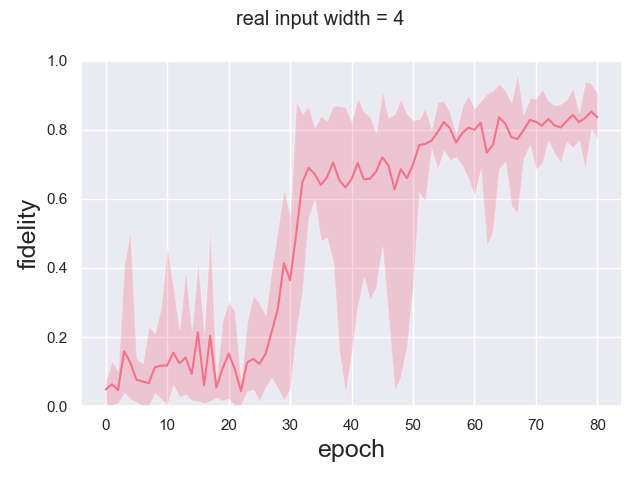
\includegraphics[width=0.3\linewidth]{figures/sqgans_size=4/fidelity.png}
  }
  \subfloat{
    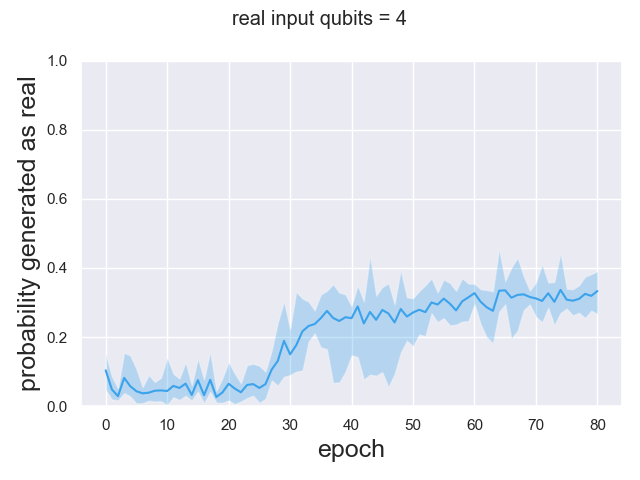
\includegraphics[width=0.3\linewidth]{figures/sqgans_size=4/probability_generated_as_real.png}
  }
  \subfloat{
    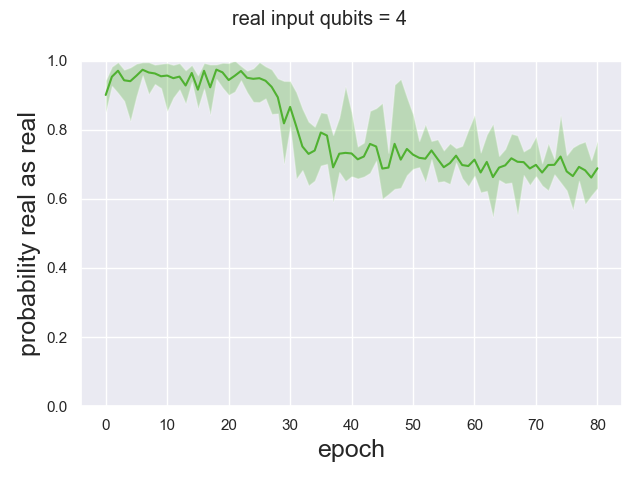
\includegraphics[width=0.3\linewidth]{figures/sqgans_size=4/probability_real_as_real.png}
  }

  \subfloat[Fidelity between real and \\generated state]{
    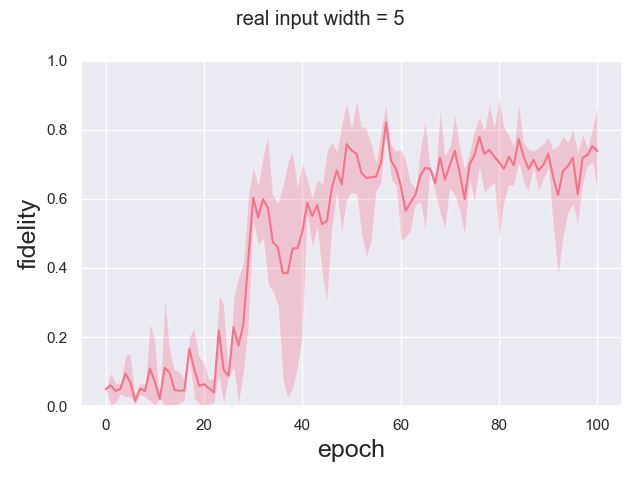
\includegraphics[width=0.3\linewidth]{figures/sqgans_size=5/fidelity.png}
  }
  \subfloat[Probability of classifying \\generated state as real]{
    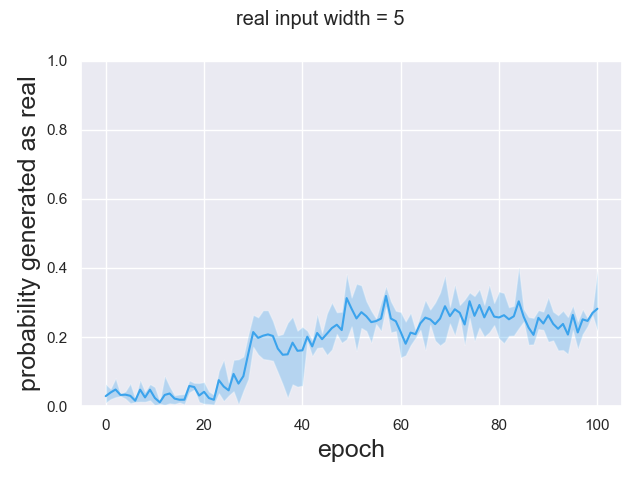
\includegraphics[width=0.3\linewidth]{figures/sqgans_size=5/probability_generated_as_real.png}
  }
  \subfloat[Probability of classifying real state as real]{
    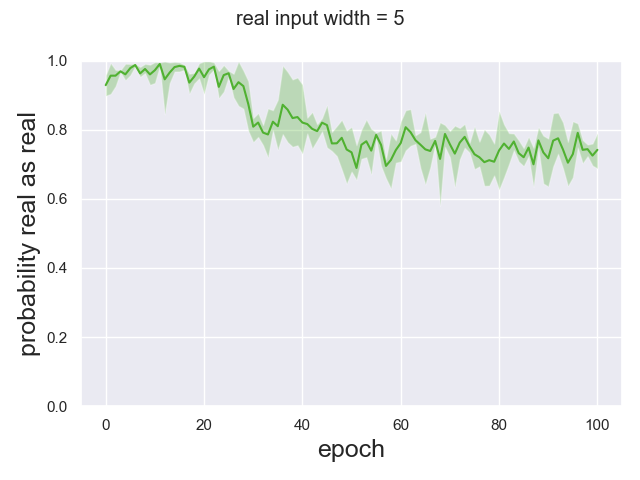
\includegraphics[width=0.3\linewidth]{figures/sqgans_size=5/probability_real_as_real.png}
  }
  \caption{The solid line represents the average value and the shaded area
    represents the range from 5 different experiments. The generator has the
    number of layers equal to the width of real input the discriminator has one
    more layer than the generator. In each epoch generator is optimized for 11 iterations and
  discriminator for 111. }
  \label{fig:sqgans_res_3}
\end{figure}
\subsubsection{Results For Mixed State Real Input}
If the real input source can provide more than one state, we can say that the
generator is learning mixed state of all the input states. Dallaire-Demers et
al. \cite{Dallaire_Demers_2018} trained a simple 2 qubits circuit with two real
input states $\ket{0}$ or $\ket{1}$. In this setup \textbf{Label} wires consist
of one qubit and also takes values $\ket{0}$ or $\ket{1}$, effectively learning
$CNOT$ gate. This strategy do not have generalize well in to more complex cases.
First, if there is more than one non-$\ket{0}$ input state, there would have to
be a separate $CNOT$ gate for each state. Second, the number of qubits necessary
for the \textbf{Label} wires grows logarithmically with the number of real input
states. Both of those cause the circuit to grow in width and depth.

Another approach we explored was to insert $R_x(\lambda_k)$ parametrized
rotation gates between each layer of the generator and discriminator. The
generator is essentially learning how to rotate input state $\ket{0}$ to some
desired real input state $\ket{r_k}$. Then, if for each $k$ the rotation is
pushed in different direction, the final generator might give different output
state for each $\lambda_k$. However, in our experiments the generator was always
learning to ignore the $R_x(\lambda_k)$ and in the end was only able to produce
one, slightly distorted, state independent of $\lambda_k$.

\subsection{Conclusions}
We have experimentally evaluated SQGANs and confirmed their ability to learn
pure quantum state. However, the problems with labeled states and small
circuit width for which the training succeeds prevented us from succeeding in
mixed state learning.

The very important aspect of generative models is ability to generate new,
unseen before, samples. In SQGANs this is theoretically possible by using the
textbf{Batch} register. However, it is not straight forward to use this register
in the intended way. First, the task of generating random quantum state is not
trivial on its own. Second, all the problems associated with the label state
$\lambda$ also apply to the random state $z$. 

Because of the above, we decided not to pursue the exploration of SQGANs further
and turned into other methods.


\section{Wasserstein Quantum GANs (WQGANs)}

As in the classical case, the WQGANs relay on calculating the Wasserstein
distance between real and generated state. However, the definition of the
Wasserstein distance cannot be trivially translated into the quantum setup.
There has been multiple approaches to defining the quantum Wasserstein distance
\cite{carlen2012analog,chen2016matrix,chen2018Wasserstein,ning2013matrixvalued,peyré2017quantum,golse2021quantum,Golse_2016,yu2019quantum},
however the first take on the Wasserstein distance in the context of quantum
GANs was proposed by Chakrabarti et. al\cite{chakrabarti2019quantum}. They
proposed the Wasserstein semi-metric and successfully used it to train the
quantum GANs. The shortcoming of this semi-metric is that, it does not preserve the
triangle inequality.


\subsection{Quantum Wasserstein Distance}
In this work, we use the definition by De Palma et.
al\cite{depalma2020quantum}. They proposed a generalization of
Wasserstein distance of order 1 into the quantum realm. The dual formulation of
this distance is stated as follows:
\begin{equation}
  W_1(\rho, \sigma) = \max_{H \in \mathcal{O}_n}{(Tr[(\rho - \sigma)H]: \norm{H}_L \leq 1
    )}.
  \label{eq:w1_distance_general}
\end{equation}
Where $\mathcal{O}_n$ is a set of all $2^n \times 2^n$ Hermitian matrices and 
$\norm{H}_L$ is the quantum Lipschitz constant of the matrix $H$ defined as:
\begin{equation}
  \norm{H}_L = 2 \max_{i=1\ldots n}{\min_{H_{\bar{i} \in \mathcal{O}_n}}{(\norm{H - H_{\bar{i}}}_\infty)}}.
\end{equation}
Where $H_{\bar{i}}$ is a Hermitian matrix that does not act on the $i$-th qubit.
The quantum Lipschitz constant and the Wasserstein distance defined in this way,
recover their classical counterparts for operators diagonal in the canonical basis.

\begin{definition}[Neighboring States]
  Two quantum states $\rho$ and $\sigma$ are Neighbouring States if they
  coincide after discarding one qubit, i.e. $\exists i: Tr_i[\rho]=Tr_i[\sigma]$
\end{definition}

Informally, the $W_1$ distance is the maximum distance that is induced by a norm
that assigns the distance at most one to any couple of Neighbouring States. 

The quantum Wasserstein distance has several properties that make it
particularly useful in the context of training the generative models.
\begin{enumerate}
\item It is invariant with respect to qubit permutations and super additive with
  respect to tensor product, (i.e. $W_1(\rho, \sigma) \geq W_1(\rho_{1 \ldots m},
  \sigma_{1 \ldots m}) + W_1(\rho_{1+m \ldots n},
  \sigma_{1+m \ldots n})$). 

  This property implies, that an operation that reduces distance between some
  marginal states also reduces the distance between the full states. For example,
  $W_1(\ket{100}, \ket{111}) > W_1(\ket{110}, \ket{111})$, this is not the case
  however for the trace distance or fidelity, as they are always $0$
  between orthogonal states. 
\item The quantum Wasserstein distance is bound by the trace distance, i.e.
  $T(\rho, \sigma) \leq W_1(\rho, \sigma) \leq nT(\rho, \sigma)$, where $n$ is
  the number of qubits. This ensures that minimizing the $W_1$ distance also
  minimizes the trace distance.
\item Because the quantum Wasserstein distance recovers classical Wasserstein
  distance for diagonal operators, we can expect that generative models build
  using this metrics preserve the advantages of their classical counterparts.
\end{enumerate}

\subsection{WQGANs Architecture}
In contract to SQGANs, the design of generator and discriminator for WQGANs
differs significantly. Here we use the architecture proposed by Kiani et. al
\cite{kiani2021quantum}. The discriminator takes a form of simple linear
program, while the generator is similar to the one for SQGANs.

\subsubsection{Discriminator}
The set $\mathcal{O}_n$ in Equation \ref{eq:w1_distance_general} is too big to
be useful in any practical scenarios. Instead the set of parametrized k-length
Pauli String is used. Specifically,
\begin{equation}
\begin{split}
  \label{eq:parametrized_hamiltonian}
  H(W) = & \sum_{i_1 = 1}^{n-k+1} \ldots \sum_{i_k = i_{k-1} + 1}^{n}\sum_{\sigma_1, \ldots, \sigma_k \in \{I, X, Y, Z\}} w^{\sigma_1,
    \ldots, \sigma_k}_{(i_1, \ldots, i_k)} \sigma^1_{i_1} \otimes \ldots \otimes \sigma^k_{i_k}  = \\
  & = \sum_{\mathcal{I}_k \subseteq \{1, \ldots, n \}} \sum_{H \in \{ I,X,Y,Z \}^{\otimes k}} w_{\mathcal{I}_k}^HH_{\mathcal{I}_k}
\end{split}
\end{equation}
Where $\mathcal{I}_k$ is a k-set of qubit indexes used to generate the k-lenght
Pauli String, $H_{\mathcal{I}_k}$ is n-length Pauli String that acts non
trivially on the set of at the most k qubits
corresponding to $\mathcal{I}_k$ and $W$ is the set of all weights.

We can also use the fact that the quantum Lipschitz constant of $H(W)$ is
bounded by:
\begin{equation}
  \label{eq:quantum_lipschitz_bound}
  \norm{H(W)}_L \leq 2 \max_{i = 1,\ldots,n}{\norm{\sum_{\{ \mathcal{I}_k: \mathcal{I}_k \subseteq \{1, \ldots, n \} \land i \in \mathcal{I}_k \}}
      \sum_{\substack{H \in \{ I,X,Y,Z \}^{\otimes k} \\
        H_{(i)} \neq I
      }} w_{\mathcal{I}_k}^HH_{\mathcal{I}_k} }_{\infty}}.
\end{equation}
Where the sum is taken only over the operators which act non-trivially on qubit
$i$\cite{kiani2021quantum}. 

To simplify the notation, the parameter set $W$ is enumerated as $W=\{w_1,
  \ldots, w_N\}$, where $N=|W|$ and $H_i$, $\mathcal{I}_{k_i}$ are Hamiltonian and index set
associated with the weight $w_i$.

Now, the equation \ref{eq:w1_distance_general} takes the form: 
\begin{equation}
  \label{eq:quantum_wasserstein_parametrized}
  W_1(\rho, \sigma) = \max_{w}{(Tr[(\rho - \sigma)\sum_{i=1}^N w_iH_i])}
\end{equation}
with the following constraint steaming from the quantum Lipschitz constant bound
from Equation \ref{eq:quantum_lipschitz_bound}.
\begin{equation}
  \label{eq:absolute_value_constraint}
\sum_{\{i: i \in \{1,\ldots, n\} \land j \in \mathcal{I}_{k_i} \}} |w_i| \leq 1, \qquad j=1,\ldots,n
\end{equation}
This optimization problem can be translated into the canonical form of linear
programming. First, let
\begin{equation}
  c_i=Tr[(\rho - \sigma)H_i],
\end{equation}  
  then Equation \ref{eq:quantum_wasserstein_parametrized} becomes
\begin{equation}
  W_1(\rho, \sigma) = \max_{w}{\sum_{i=1}^N w_ic_i}.
\end{equation}  
Then, with
\begin{equation}
    w_i = w_i^+ - w_i^-
\end{equation}
the absolute value constraint from Equation \ref{eq:absolute_value_constraint} is equivalent to the following set of
constraints: 
\begin{equation}
\begin{split}
  w_i^+ &\ge 0 \\
  w_i^- &\ge 0 \\
  \sum_{\{i: i \in \{1,\ldots, n\} \land j \in \mathcal{I}_{k_i} \}} (w_i^+ + w_i^-) &\leq 1, \qquad j=1,\ldots,n
\end{split}
\end{equation}
Now, with two vectors defined as:
\begin{equation}
\begin{split}
\bm{w'} &= [w_1^+, w_1^-, \ldots, w_N^+, w_N^-] \\
\bm{c'} &= [c_1, -c_1, \ldots, c_N, -c_N],
\end{split}
\end{equation}
matrix $A^{n \times N}$ defined as:
\[A_{j, i}  = \begin{cases} 
    1 & \text{if} \quad j \in \mathcal{I}_{k_i} \\
    0 & \text{else}
  \end{cases}
\]
The discriminator linear program in the canonical form looks as follows:
\begin{equation}
\begin{split}
  \max_{\bm{w'}}{} \quad & \bm{c'}^T \bm{w'}\\
  \text{subject to } \quad & \bm{w'} \geq \bm{0} \\
  & A\bm{w'} \leq \bm{1}.
\end{split}
\end{equation}

The weights from the original set $W$ are recovered as:
\begin{equation}
  w_i = w_{2i-1}' - w_{2i}'.
\end{equation}


The linear program with $n$ constraints outputs at most $n$ non-zero
weights\cite{10.5555/548834}, so the optimal Hamiltonian which approximates the
quantum Wasserstein distance the best is given by:
\begin{equation}
\hat{H} = \sum_{i=1}^{\hat{N}}\hat{w}_i\hat{H}_i,
\end{equation}
Where $\hat{N} \leq n$.

The Hamiltonian obtained in this way acts as the ``discriminator'' and it used
to train the generator in the typical minmax game of GANs.

\subsubsection{Generator}
Similarly to SQGANs, the generator is built using parametrized quantum circuits.
Specifically, the generator is defined as a sum of parametrized quantum circuits
with corresponding probabilities:
\begin{equation}
G(\theta) = \sum_{i=1}^r p_iG_i(\theta_i)\rho_0G_i(\theta_i)^\dagger.
\end{equation}
Where $\sum_{i=1}^r p_i = 1$ and $p_i$ is the probability associated with the
circuit $G_i$ and $\rho_0$ is the initial state of the circuit. The summation is
essentially the maximal rank of the output state that the generator is able to
generate. Namely, the generator constructed like that is able to learn a mix of
at most $r$ pure states.

In all of our experiments we use the same design for each circuit within the
generator, i.e. $G_i = \bar{G} \quad \forall i \in 1,\ldots, r$, and only the
parameters $\theta_i$ differ. We use different designs for $\bar{G}$ for
different experiments, however they always fall into two categories.
\begin{enumerate}
\item Generic $\bar{G}$ described in Appendix \ref{apx:sqgans_ansatz} (the same as for SQGANs).
\item $\bar{G}$ the same as the circuit used to generate the real input state.
\end{enumerate}
We also always set the initial state $\rho_0 = \ket{0}$.

In the end the generator becomes:
\begin{equation}
  G(\theta) = \sum_{i=1}^r p_i\bar{G}(\theta_i)\ket{0}\bar{G}(\theta_i)^\dagger.
\end{equation}



\subsection{Training}
Similarly to WGANs the discriminator part of the WQGANs computes the best
approximation of the quantum Wasserstein distance and the generator tries to
minimize it. This can be again encoded as the minmax game.

Given real input state $\rho_r$, generated state $G(\theta)$ and using trace
properties from Equation \ref{eq:quantum_wasserstein_parametrized} we get:

\begin{equation}
  \label{eq:quantum_wasserstein_separated_trace}
  \begin{split}
    W_1(\rho_r, G(\theta)) = \max_{w}{(Tr[(\rho_r - G(\theta))\sum_{i=1}^N w_iH_i])} = \max_{w}{(\sum_{i=1}^Nw_i(Tr[\rho_rH_i] - Tr[G(\theta)H_i]))}.
  \end{split}
\end{equation}
The generator tries to minimize the quantum Wasserstein distance to the real
input state, so in general terms WQGANs optimization objective is stated as:
\begin{equation}
  \max_{w}{\min_{\theta}{\mathcal{L}(w, \theta)}} = \max_{w}{\min_{\theta}{(\sum_{i=1}^Nw_i(Tr[\rho_rH_i] - Tr[G(\theta)H_i]))}} 
\end{equation}
In practice however, we do not have to calculate the expectation $Tr[G(\theta)H_i]$ for
every $i$ when training the Generator, instead we can use the $\hat{H}$ defined
earlier. Also, the real input state expectations $Tr[\rho_rH_i]$ can be
precomputed and only accessed during the training.

The overall training procedure consists of the following steps:
\begin{enumerate}
\item Compute the expectations $Tr[G(\theta)H_i]$ and use them together with
  the precomputed expectation for the real input state to calculate $Tr[\rho_rH_i] -
  Tr[G(\theta)H_i]$ for each $i$.
\item Find $\hat{H}$ using the linear programming formulation.
\item Use $\hat{H}$ to find gradients of $Tr[G(\theta)\hat{H}]$ w.r.t parameters
  $\theta_i$ and $p_i$ and update them.
\end{enumerate}

Those 3 steps are repeated until some stopping condition is satisfied, in our
case we run the training for given number of steps.

\subsection{Evaluation Results}
\subsubsection{Experimental Setup}
We use two different circuits to generate real input samples. First one is the
same as used in the SQGANs and is described in Appendix
\ref{apx:topological_phase_transition_ansatz}.
The second one is a butterfly circuit (also used by Kiani et.
al\cite{kiani2021quantum}) which is described in Appendix
\ref{apx:butterfly_ansatz}. For the butterfly circuit we use random
initialization for all the gates.

We try two different approaches to the generator design. We use the generic
generator described in Appendix \ref{apx:sqgans_ansatz} and generator
design matching the circuit used to generate real input data. We specify the
details of generator architecture for each experiment separately.

In all the experiment we use Adam optimizer \cite{kingma2017adam} with
parameters $\beta_1 = 0.9$, $\beta_2=0.98$, $\hat{\epsilon} = 1e-9$ and the
learning rate of $0.1$. This learning rate was determined by experimentally. It
is important to note that the training procedure is very sensitive to changes to
this parameter. If the learning rate is too low, gradient very quickly falls in
a local optimum and the fidelity between real and generated state stays close to $0$.

The generator and discriminator are trained interchangeably one iteration each
and the exact number of epoch is specified for each experiment separately.
\subsubsection{Results For Pure Real State}
First we look at the results for topological phase transition estimation in
Figure \ref{fig:wqgans_res_1}. The real input state is generated by running the circuit from Appendix
\ref{apx:topological_phase_transition_ansatz} for random $g \in [-1; 1]$ and the
generator is built using the generic ansatz from Appendix
\ref{apx:sqgans_ansatz}. Again, no surprisingly the training gets more difficult
as the real input size grows.

Two the most impactful training parameters are the number of
generator layers and k-length of Pauli strings used in the discriminator. With
$k=3$ the fidelity is larger than $0.9$ for real input size up to $6$ qubits.
For bigger real input sizes, expectation of larger operator is needed. The convergence is
very fast, for $4$ generator layers only around $100$ epoch are necessary to
achieve very good approximation, the improvements beyond that are rather
minimal. For $5$ layers the training must be longer and it's much harder to
achieve high fidelity. For more results refer to Appendix \ref{apx:wqgans_pahse_results}.



\begin{figure}[htbp!]
  \captionsetup[subfigure]{labelformat=empty}
  \centering
  \subfloat{
    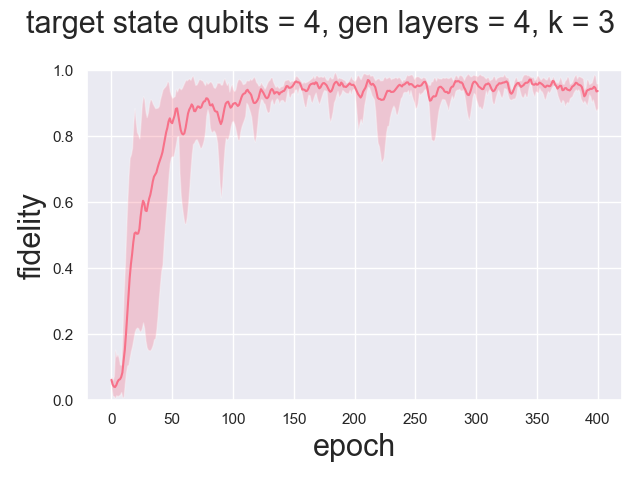
\includegraphics[width=0.25\linewidth]{figures/wqgans_phase_size=4_k=3_gen=4/fidelity.png}
  }
  \subfloat{
    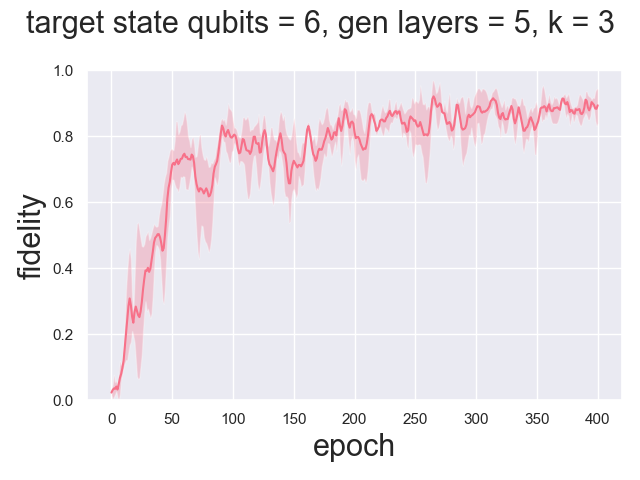
\includegraphics[width=0.25\linewidth]{figures/wqgans_phase_size=6_k=3_gen=5/fidelity.png}
  }
  \subfloat{
    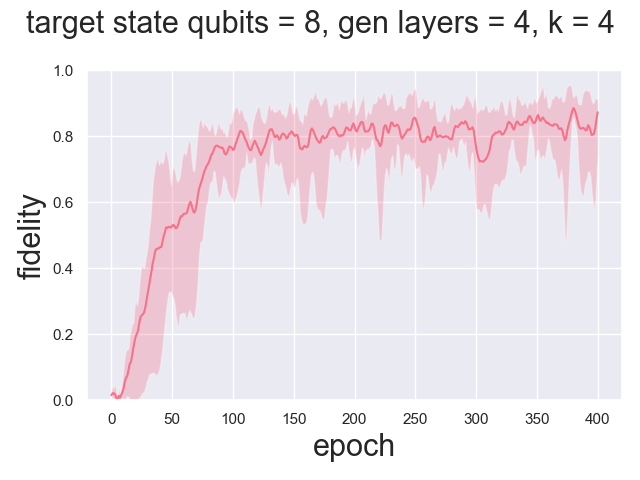
\includegraphics[width=0.25\linewidth]{figures/wqgans_phase_size=8_k=4_gen=4/fidelity.png}
  }
  \subfloat{
    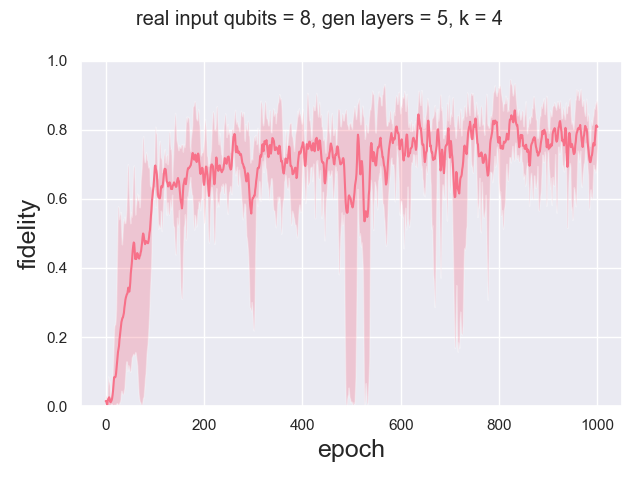
\includegraphics[width=0.25\linewidth]{figures/wqgans_phase_size=8_k=4_gen=5/fidelity.png}
  }

  \subfloat{
    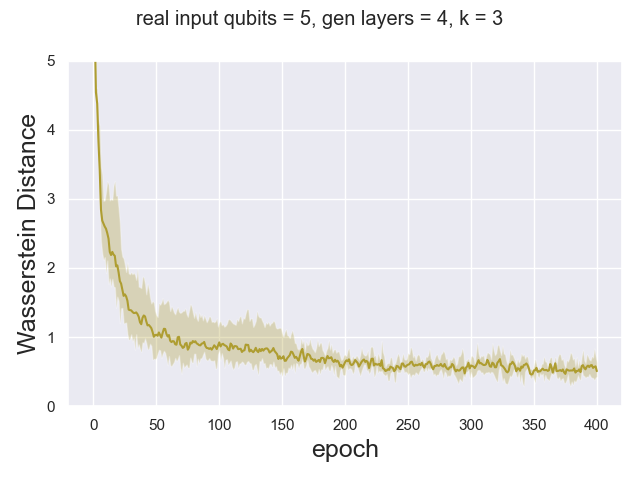
\includegraphics[width=0.25\linewidth]{figures/wqgans_phase_size=5_k=3_gen=4/Wasserstein_Distance.png}
  }
  \subfloat{
    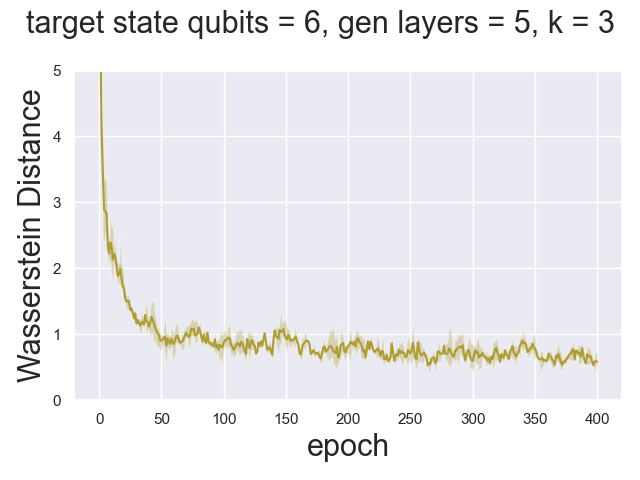
\includegraphics[width=0.25\linewidth]{figures/wqgans_phase_size=6_k=3_gen=5/Wasserstein_Distance.png}
  }
  \subfloat{
    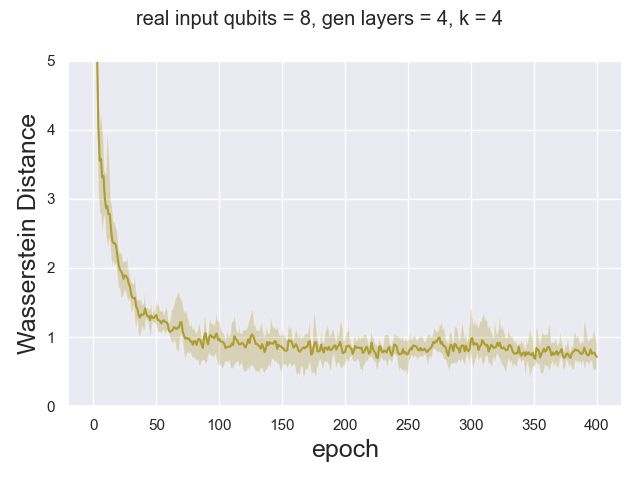
\includegraphics[width=0.25\linewidth]{figures/wqgans_phase_size=8_k=4_gen=4/Wasserstein_Distance.png}
  }
  \subfloat{
    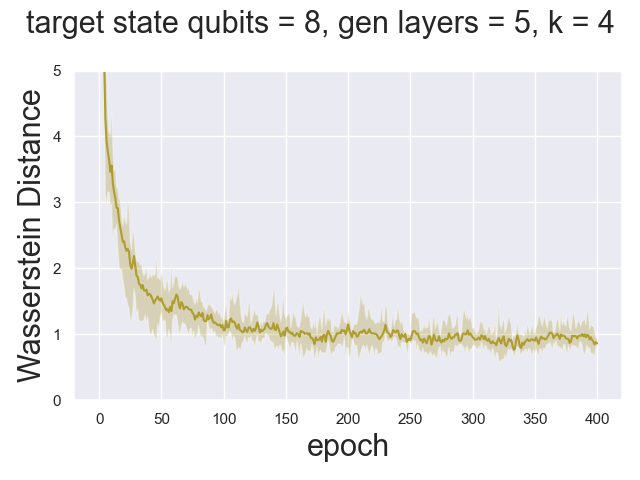
\includegraphics[width=0.25\linewidth]{figures/wqgans_phase_size=8_k=4_gen=5/Wasserstein_Distance.png}
  }
  \caption{Results of topological phase transition estimation (ansatz Appendix \ref{apx:topological_phase_transition_ansatz}).
    The solid line represents the average value and the shaded area
    represents the range from 5 different experiments. The upper row shows the
    fidelity and the bottom row shows the corresponding Wasserstein distance. In all the
    experiments the generator is built using ansatz from \ref{apx:sqgans_ansatz}.}
  \label{fig:wqgans_res_1}
\end{figure}


The results for the butterfly circuit estimation are shown in the Figure
\ref{fig:wqgans_res_butterfly_1}. The real input state is generated by running
the circuit from Appendix \ref{apx:butterfly_ansatz} for randomly selected
values in each gate and the generator is built using the generic ansatz from Appendix
\ref{apx:sqgans_ansatz}. Again, no surprisingly the training gets more difficult
as the real input size grows. However, in this case we can see that the results
are worse than for the phase transition circuit.


\begin{figure}[htbp!]
  \captionsetup[subfigure]{labelformat=empty}
  \centering
  \subfloat{
    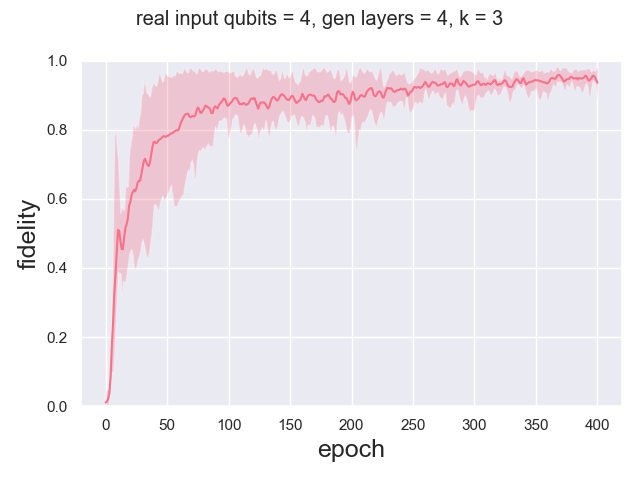
\includegraphics[width=0.25\linewidth]{figures/wqgans_butterfly_size=4_k=3_gen=4/fidelity.png}
  }
  \subfloat{
    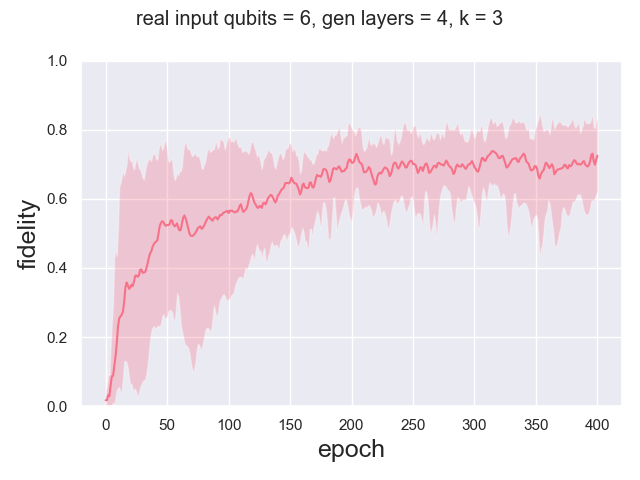
\includegraphics[width=0.25\linewidth]{figures/wqgans_butterfly_size=6_k=3_gen=4/fidelity.png}
  }
  \subfloat{
    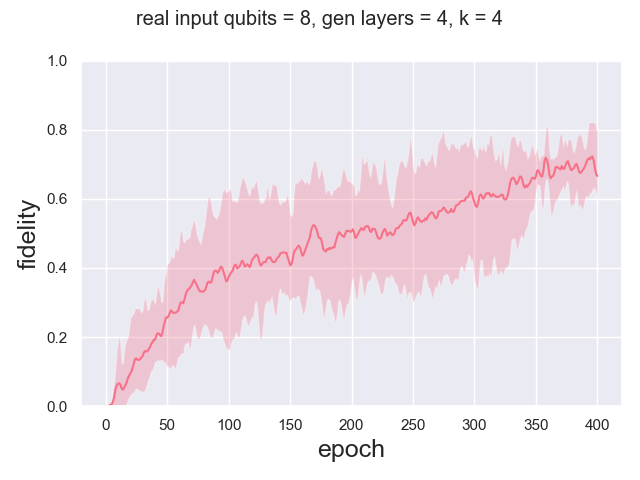
\includegraphics[width=0.25\linewidth]{figures/wqgans_butterfly_size=8_k=4_gen=4/fidelity.png}
  }
  \subfloat{
    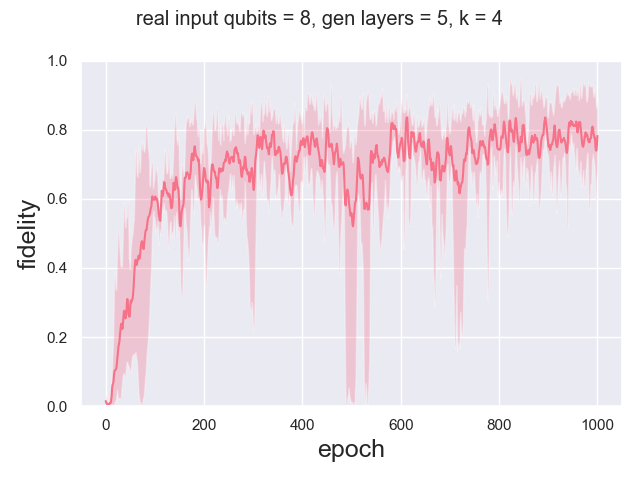
\includegraphics[width=0.25\linewidth]{figures/wqgans_butterfly_size=8_k=4_gen=5/fidelity.png}
  }

  \subfloat{
    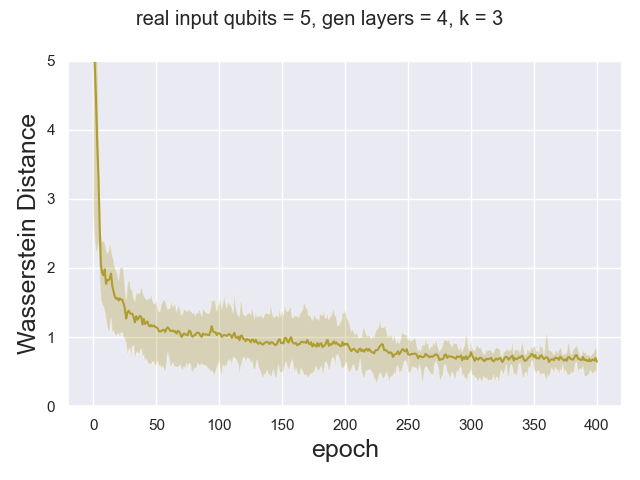
\includegraphics[width=0.25\linewidth]{figures/wqgans_butterfly_size=5_k=3_gen=4/Wasserstein_Distance.png}
  }
  \subfloat{
    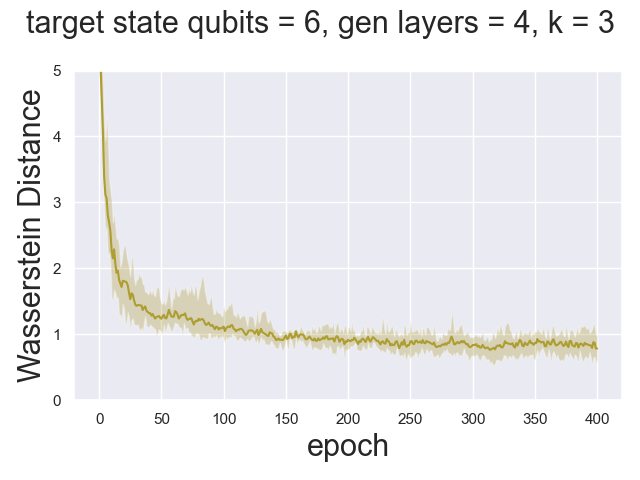
\includegraphics[width=0.25\linewidth]{figures/wqgans_butterfly_size=6_k=3_gen=4/Wasserstein_Distance.png}
  }
  \subfloat{
    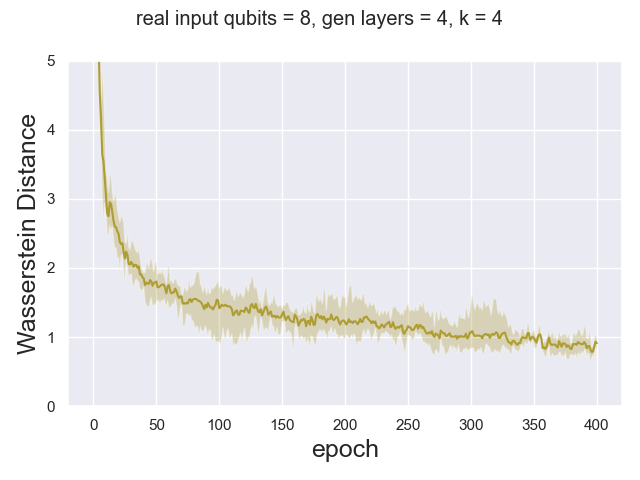
\includegraphics[width=0.25\linewidth]{figures/wqgans_butterfly_size=8_k=4_gen=4/Wasserstein_Distance.png}
  }
  \subfloat{
    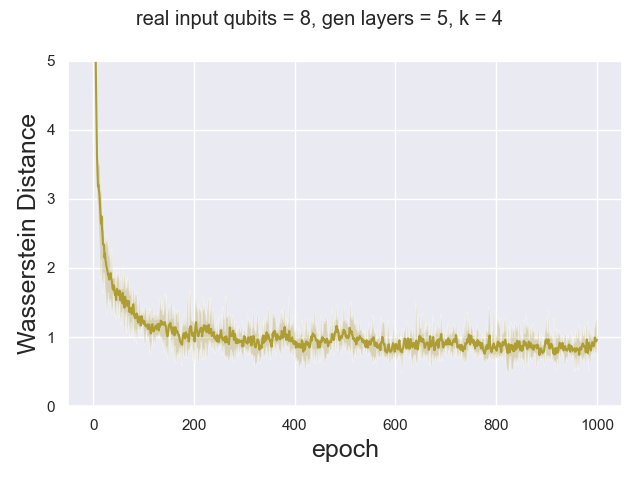
\includegraphics[width=0.25\linewidth]{figures/wqgans_butterfly_size=8_k=4_gen=5/Wasserstein_Distance.png}
  }
  \caption{Results for butterfly circuit (ansatz Appendix \ref{apx:butterfly_ansatz}).
    The solid line represents the average value and the shaded area
    represents the range from 5 different experiments. The upper row shows the
    fidelity and the bottom row shows the corresponding Wasserstein distance. In all the
    experiments the generator is built using ansatz from \ref{apx:sqgans_ansatz}.}
  \label{fig:wqgans_res_butterfly_1}
\end{figure}

It is interesting to compare those results, with the one obtained using the
same circuit ansatz for both, real input and the generator. In Figure
\ref{fig:wqgans_res_butterfly_same} we see the results for using the butterfly
circuit for both, real input and generator. Regardless of the size, very high
fidelity was achieved. This shows the importance of the generator design in the
training process.


\begin{figure}[htbp!]
  \captionsetup[subfigure]{labelformat=empty}
  \centering
  \subfloat{
    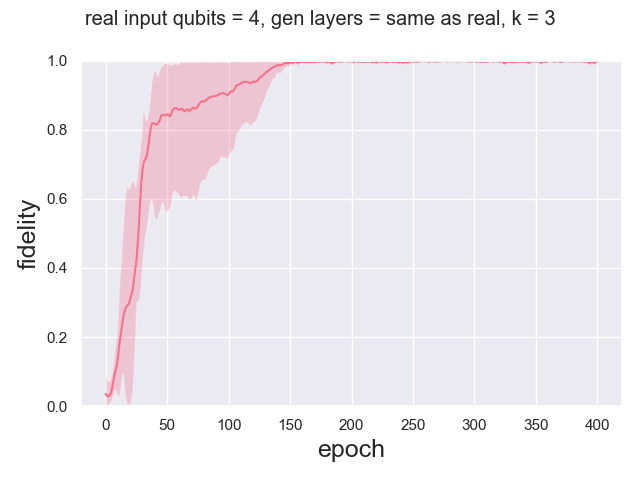
\includegraphics[width=0.25\linewidth]{figures/wqgans_butterfly_size=4_k=3_gen=same_as_real/fidelity.png}
  }
  \subfloat{
    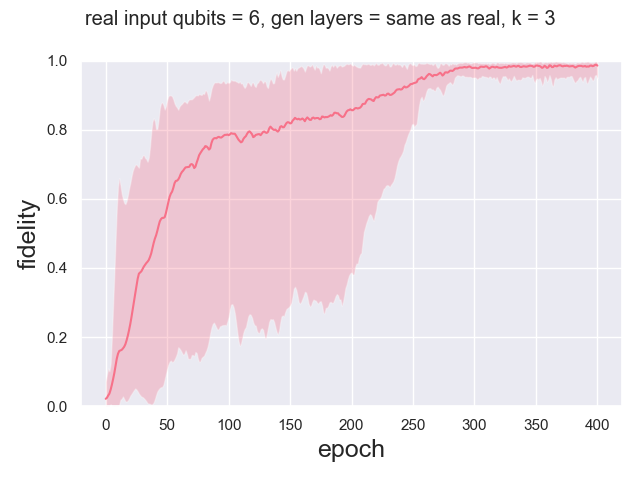
\includegraphics[width=0.25\linewidth]{figures/wqgans_butterfly_size=6_k=3_gen=same_as_real/fidelity.png}
  }
  \subfloat{
    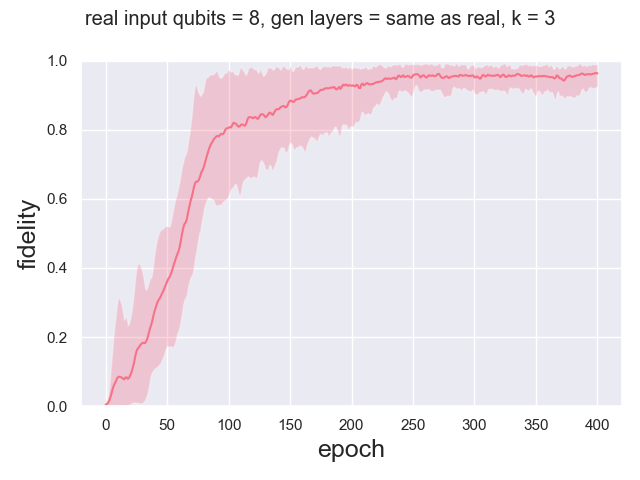
\includegraphics[width=0.25\linewidth]{figures/wqgans_butterfly_size=8_k=3_gen=same_as_real/fidelity.png}
  }
  \subfloat{
    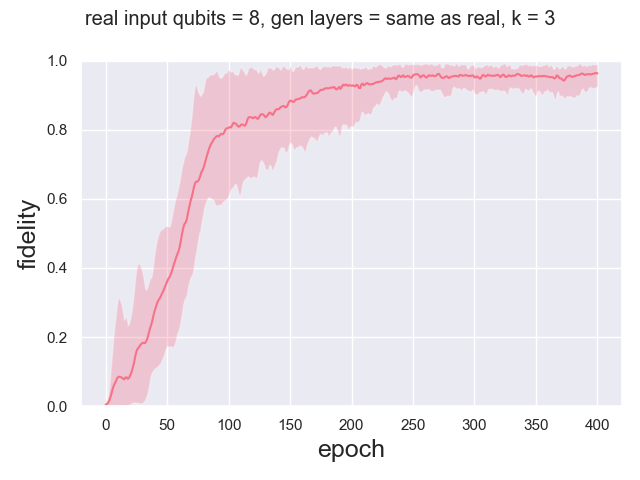
\includegraphics[width=0.25\linewidth]{figures/wqgans_butterfly_size=8_k=3_gen=same_as_real/fidelity.png}
  }

  \subfloat{
    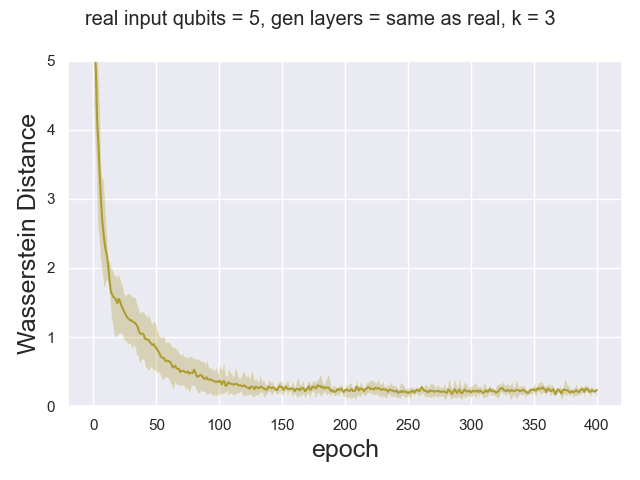
\includegraphics[width=0.25\linewidth]{figures/wqgans_butterfly_size=5_k=3_gen=same_as_real/Wasserstein_Distance.png}
  }
  \subfloat{
    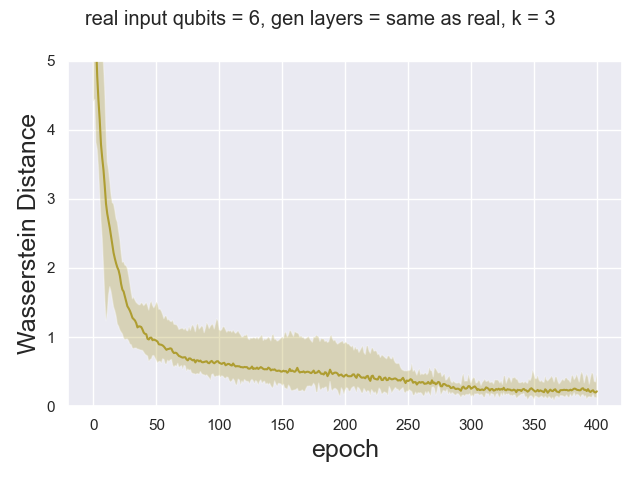
\includegraphics[width=0.25\linewidth]{figures/wqgans_butterfly_size=6_k=3_gen=same_as_real/Wasserstein_Distance.png}
  }
  \subfloat{
    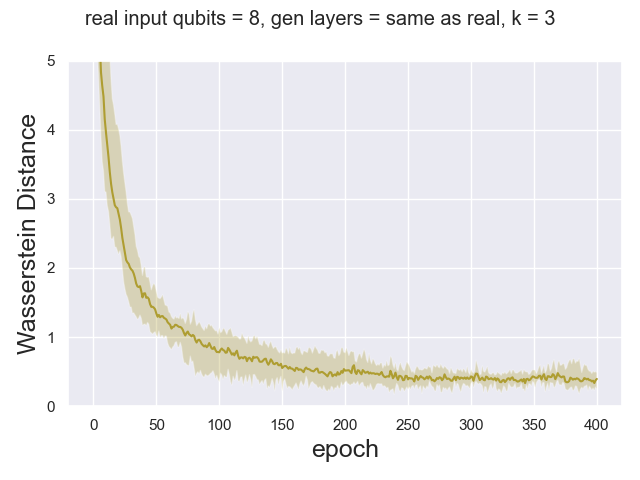
\includegraphics[width=0.25\linewidth]{figures/wqgans_butterfly_size=8_k=3_gen=same_as_real/Wasserstein_Distance.png}
  }
  \subfloat{
    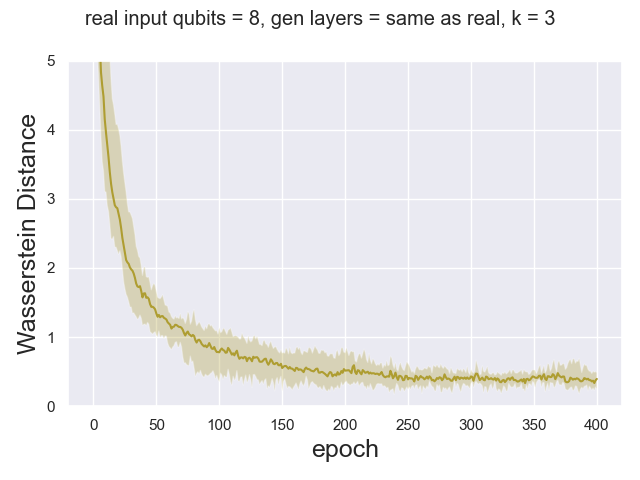
\includegraphics[width=0.25\linewidth]{figures/wqgans_butterfly_size=8_k=3_gen=same_as_real/Wasserstein_Distance.png}
  }
  \caption{Results for butterfly circuit (ansatz Appendix \ref{apx:butterfly_ansatz}).
    The solid line represents the average value and the shaded area
    represents the range from 5 different experiments. The upper row shows the
    fidelity and the bottom row shows the corresponding Wasserstein distance. In all the
    experiments the generator is built using the same butterfly circuit.}
  \label{fig:wqgans_res_butterfly_same}
\end{figure}


In all the examples we see that the approximated Wasserstein distance approaches $0$
as fidelity approaches $1$, which is the expected behavior. The Wasserstein
distance below $1$ indicates high fidelity between real input and generated
states.

It is also important to note here, that using fixed $k$ might not be optimal
strategy. If for given operator, the different between expectation of the
generator and the real input source is close to $0$, this operator does not
provide any useful information in context of learning anymore. So instead of
evaluating all operators for given $k$, we can start with some subset and
remove and add new ones as the training progresses \cite{kiani2021quantum}. 
\subsubsection{Results For Mixed Real State}
The generator definition allows for mixed state approximation. In theory each
circuit in the generator should be able to learn different pure state and its
probability in the mix. However, we found it difficult to achieve in practice.

We did not manage to train mixed state generator using the generic ansatz. But
when using the same ansatz for the real input and the generator we were able
approximate an equal mixture of two topological phase transition circuits (results
presented in Figure \ref{fig:wqgans_grid_phase_1}). The generator with 4 circuits
used 2 of them to approximate the real input and also learnt the correct
probability of $0.5$ for both of them. The other 2 circuits got assigned the
probability close to $0$ and states far from the one in the real input.

\begin{figure}[htbp!]
  \captionsetup[subfigure]{labelformat=empty}
  \centering
  \subfloat{
    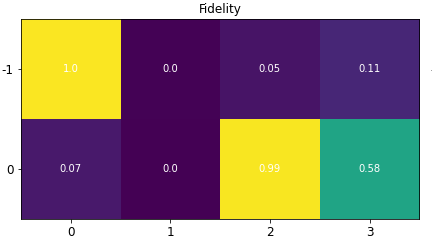
\includegraphics[width=0.5\linewidth]{figures/fidelity_grid_phase.png}
  }
  \subfloat{
    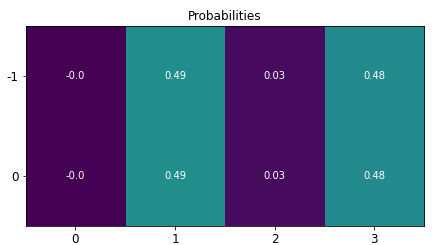
\includegraphics[width=0.5\linewidth]{figures/prob_grid_phase.png}
  }
  \label{fig:wqgans_grid_phase_1}
  \caption{Results for topological phase transition circuit (Appendix
    \ref{apx:topological_phase_transition_ansatz}). The real input source
    produces two states (for $g=0$ and $g=-1$) each with $0.5$ probability.
    The generator consist of 4 circuits, each with the same ansatz as the real
    input. (left) the circuit with index $0$ learnt the state for $g=-1$ and the
    circuit with index $2$ learnt the state for $g=0$. The other two circuits
    did not any of the states well. (right) How far is the probability of given
    circuit from the actual probability in the real input. For the circuit $0$
    and $2$ the number is close to $0$, which means that the probability was
    correctly learnt to be $0.5$, for the other two it's close to $0.5$, which
    means it is correctly around $0$.
  }
\end{figure}

The results for the mixture of 3 states in the real input were much worse. While
there were signs that the generator was learning, usually one of the
states was forgotten (i.e. the generator learnt only the mixture of 2 states).

\subsubsection{Conclusions}
Our experiments confirmed the ability to approximate quantum states using the
quantum Wasserstein distance. It is easier to train such networks and they give
better results than SQGANs. As the input size grows, increasing the Pauli
Strings length $k$ allows for high approximation (at the cost of increased
training complexity).

The design of the generator plays a crucial role in the quality of the
approximations. Better design also allows to use lower $k$ which makes the
training more efficient.

WQGANs also work for mixed state approximation, although only for small
mixtures.

However, this architecture still does not allow to generate new, unseen before,
states. In the next chapter we explore ways in which this can be achieved using WQGANs. 

%%% Local Variables:
%%% mode: latex
%%% TeX-master: "../main"
%%% End: